%%%%%%%%%%%%%%%%%%%%%%%%%%%%%%%%%%%%%%%%%%%%%%%%%%%%%%%%%%%%%%%%%%%%%%%%
%                                                                      %
%     File: Thesis_Results.tex                                         %
%     Tex Master: Thesis.tex                                           %
%                                                                      %
%     Author: Andre C. Marta                                           %
%     Last modified :  2 Jul 2015                                      %
%                                                                      %
%%%%%%%%%%%%%%%%%%%%%%%%%%%%%%%%%%%%%%%%%%%%%%%%%%%%%%%%%%%%%%%%%%%%%%%%

\chapter{V-F Optimization Mechanism}
\label{chapter:mech}


The results from the previous chapter display that the energy-efficiency (through the \acrshort{edp}) of an out-of-the-shelf \acrshort{gpu} can be significantly improved if a specific non-conventional V-F pair is applied on the Core \acrshort{dvfs} domain. 

However, in the previous chapter, one does not perform the frequency and voltage scaling dynamically, being one of the dissertation's objectives.
To address this dynamic tunning of frequency and voltage while using the increased exploration space (and taking into account that it is necessary to guarantee safe \acrshort{gpu} operation), two approaches can be followed: creating a forecasting model or creating an online optimization mechanism.

The forecasting model would predict the V-F pair to use based on the executing code (analysis of the Assembly code) and performance counters (the trace of the application being executed). This option has the benefit of allowing the complete execution of the target application under the best possible configuration. However, such a forecasting model would also have to take into consideration the \acrshort{gpu} temperature, utilization (the target application being executed by itself or concurrently with others) and more importantly, it would be very tied to a specific \acrshort{gpu} model. In so, this option would become complicated and not easily scalable between different \acrshort{gpu}s.

On the other hand, the online optimization mechanism can target the native code repetition on \acrshort{gpgpu} applications solving algorithms. For these applications, the best overall configuration is the best V-F pair for each algorithm's step. In algorithms where the time it takes to perform a step is significantly shorter than the time it takes to compute the total algorithm, it is possible to discover and achieve the optimal V-F configuration quickly. This approach has the added advantage of optimizing the \acrshort{gpu} for their current state: temperature, utilization, aging and all \acrshort{pvt} variation.

Due to the benefits of targeting the current \acrshort{gpu} state, the second approach, the creation of an online V-F optimization mechanism, is followed. This chapter provides an overview of the optimization mechanism and explains how it should be adapted to the target application.


%%%%%%%%%%%%%%%%%%%%%%%%%%%%%%%%%%%%%%%%%%%%%%%%%%%%%%%%%%%%%%%%%%%%%%%%
\section{V-F Optimization Mechanism description}
\label{section:opt}

The devised V-F optimization mechanism follows the block diagram of Figure~\ref{fig:opt_mech}, consisting of a two-phase process. The following sections provide an in-depth explanation of each step of the mechanism, clarifying its objectives and requirements.

\begin{figure}[htb]
  \centering
  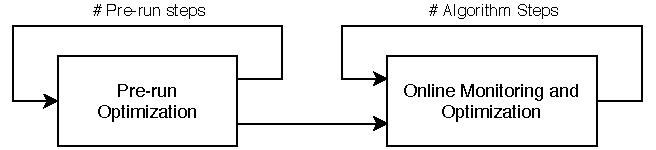
\includegraphics[width=0.75\textwidth]{Figures/Optimization/full_mech_2.pdf}
  \caption{V-F Optimization Mechanism Block Diagram.}
  \label{fig:opt_mech}
\end{figure}

\subsection{Objective and Requirements}

The V-F optimization mechanism aims to discover and achieve the optimal V-F configuration to the running \acrshort{gpgpu} application and current \acrshort{gpu} state, optimizing for \textit{performance}, \textit{energy consumption} or \textit{energy-efficiency} (\acrshort{edp}). This optimal V-F configuration depends on the type of computations being performed, the \acrshort{gpu} temperature, utilization and aging and is selected from an exploration space concluded from the set of experiments covered on chapter~\ref{chapter:gpu_char}. 

The envisioned optimization mechanism is better suited to \acrshort{gpgpu} applications with a native code repetition - iterative algorithms like the training of deep neural networks. In particular, to applications where each iteration step takes significantly less time to compute than the algorithm's total computation time. This requirement is not mandatory; however, applications that follow this pattern can more significantly benefit from the mechanism since it can find the most appropriate configuration faster.

Another important characteristic of the optimization mechanism is that it takes into account the time that the voltage frequency controllers of regular \acrshort{gpu}s take to change these parameters. It is better and safer to allow a portion of time between V-F changes, guaranteeing that the control mechanism has time to perform the change and stabilize both the frequency as well as the voltage before continuing to execute the computation.


\subsection{Architecture Overview}

The devised mechanism is comprised of a two-phase process, that in order, tries to find the V-F configuration that achieves the highest \textit{performance}, lowest \textit{energy consumption}, or best \textit{energy efficiency} for the running application. Targeting the dissertation objective, the chosen and exemplified metric from now on is \textit{energy efficiency} through the \acrshort{edp}, computed as 
\begin{equation}
	EDP=energy * computation \: time.
	\label{eq:edp}
\end{equation}
By changing the applied Core V-F configuration, the \acrshort{edp} value is increased or decreased, allowing for comparing if the new configuration is better than the old. 

Each phase of the optimization mechanism follows the block diagram of Figure~\ref{fig:detail_mech}. Before executing the algorithm step, the energy and computation time calculation is started. After the step is concluded, the energy and computation time are computed, and in addition to specific application status, the results are provided for the optimization mechanism. The optimization mechanism is responsible for comparing the last \acrshort{edp} result with the best available, accept or reject the new configuration, and generate a new one for the next application epoch. It also analyses the application output to guarantee if the current volta-frequency pair allows correct \acrshort{gpu} computations.

\begin{figure}[htb]
  \centering
  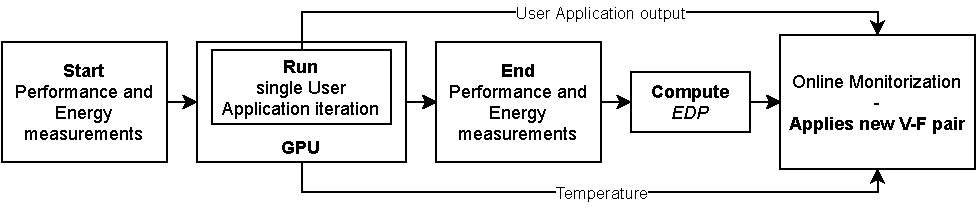
\includegraphics[width=0.75\textwidth]{Figures/Optimization/opt_pre_run.pdf}
  \caption{Pre-Run V-F Optimization Mechanism Block Diagram.}
  \label{fig:detail_mech}
\end{figure}

\subsubsection{Pre-run Optimization}

The optimal configuration can vary dramatically due to the complex behavior of the different architectural components when subjects to different workloads. With so, the objective of the first phase, \textit{Pre-run Optimization}, is to be able to find the global minimum of the exploration space, without testing all the possible configurations (as performed on Chapter~\ref{chapter:gpu_char}). To do so, it applies the \textit{Simulated Annealing} algorithm to accept or reject a new V-F configuration based on the computed \acrshort{edp} value. This algorithm excels at finding an approximate global optimum in a fixed amount of time. 

At the beginning of the execution, the \acrshort{gpu} is set to the highest default performance level. The achieved \acrshort{edp} result acts as a baseline to which all following values are normalized to. After each optimization step, a new frequency and voltage configuration are generated.
The new frequency of the new configuration is any of the available default frequencies, and the possible selected voltage is selected by looking at the valid voltage exploration space for the given frequency, discretizing the voltage range in $25mV$ steps.
For each optimization step, if the new \acrshort{edp} value is smaller than the previous, the configuration is accepted. If the result is worst, the configuration is accepted based on the \textit{Simulated Annealing} algorithm.

If, after $ N $ execution steps, a no better configuration is found, or the predefined \textit{Pre-Run Steps} is concluded, the \textit{Pre-run Optimization} is ended, with the best V-F configuration being selected for the algorithm execution.

\subsubsection{Online Monitoring Optimization}

After the execution of the \textit{Pre-run Optimization}, a quasi-optimal configuration is found. The objective of the textit{Online Monitoring Optimization} is to achieve the best possible configuration while monitoring the application status to guarantee the correct application output. The overall scheme of this phase is similar to the first one. However, in this case, the \textit{Hill Climbing} algorithm is used instead. This algorithm only accepts a new configuration if it is able to further minimize the \acrshort{edp} value, being specialized in finding the global optimization minimum having the certainty that it is on the neighborhood of the initial phase V-F configuration. For it, the new frequency configuration can be $-10Mhz$, equal or $+10MHz$ than the current one, with the voltage following the same principle, being $-10mV$, equal or $+10mV$ than the current one.
The online monitoring phase cames in action in two forms. First, it applies a temperature undervoltage behavior model, presented in Section~\ref{sec:temp_model},  that minimizes the currently applied undervoltage when the temperature increases, to guarantee correct \acrshort{gpu} operation under all conditions. Second, it monitors the application output. After each algorithm step's execution, if an invalid application output is found, the undervoltage is decreased by $10mV$, guaranteeing that the V-F configuration does not induce the current invalid output. This policy acts as a fail-safe that should not be necessary if a valid exploration space and temperature model are acquired for the present \acrshort{gpu}.



\section{Summary}